\renewcommand{\theequation}{\theenumi}
\renewcommand{\thefigure}{\theenumi}
\begin{enumerate}[label=\thesubsection.\arabic*.,ref=\thesubsection.\theenumi]
\numberwithin{equation}{enumi}
\numberwithin{figure}{enumi}
%
\item What conics do the following equation represent? When possible, find the centres and also their equations referred to the centre

\begin{align}
12x^2-23xy+10y^2-25x+26y=14\label{eq:solutions/40/1/ques}
\end{align}
\\
\solution
The given equation \eqref{eq:solutions/40/1/ques} can be expressed as 
\begin{align}
&\vec{x}^T\myvec{12 & \frac{-23}{2}\\\frac{-23}{2} & 10}\vec{x}+2\myvec{\frac{-25}{2} & 13}\vec{x}-14=0\label{eq:solutions/40/1/given}
\end{align}

where 
\begin{align}
\vec{V}&=\myvec{12 & \frac{-23}{2}\\\frac{-23}{2} & 10}\\
\vec{u}&=\myvec{\frac{-25}{2} \\ 13}\\
f&=-14
\end{align}

\begin{align}
    \det(\vec{V})&=\begin{array}{|cc|}
12 & \frac{-23}{2}\\\frac{-23}{2} & 10
\end{array}\\
\implies\det(\vec{V})&=\frac{-49}{4}\\
\implies\det(\vec{V})&<0
\end{align}

Since $\det(\vec{V})<0$ the given equation \eqref{eq:solutions/40/1/given} represents the hyperbola
The characteristic equation of $\vec{V}$ is obtained by evaluating the determinant 

\begin{align}
       \begin{array}{|c|}
V-\lambda\vec{I}
\end{array}&=0\\
   \begin{array}{|cc|}
12-\lambda & \frac{-23}{2} \\ \frac{-23}{2} & 10-\lambda
\end{array}&=0\\
\implies 4\lambda^2-88\lambda-49&=0\label{eq:solutions/40/1/eqroots}
\end{align}

The eigenvalues are the roots of equation \ref{eq:solutions/40/1/eqroots} is given by 
\begin{align}
    \lambda_1&=\frac{22+\sqrt{533}}{2}\label{eq:solutions/40/1/eqeig1}\\
    \lambda_2&=\frac{22-\sqrt{533}}{2}\label{eq:solutions/40/1/eqeig2}
\end{align}

The eigenvector $\vec{p}$ is defined as 
\begin{align}
    \vec{V}\vec{p}&=\lambda\vec{p}\\
    \implies (\vec{V}-\lambda\vec{I})\vec{p}&=0\label{eq:solutions/40/1/eqev}
\end{align}

For $\lambda_1=\frac{22-\sqrt{533}}{2}$ ,
\begin{align}
    (\vec{V}-\lambda_1\vec{I})=\myvec{\frac{\sqrt{553}+2}{2} & \frac{-23}{2} \\\frac{-23}{2} & \frac{\sqrt{533}-2}{2}}
\end{align}

By row reduction , 
\begin{align}
    &\myvec{\frac{\sqrt{533}+2}{2} & \frac{-23}{2} \\\frac{-23}{2} & \frac{\sqrt{533}-2}{2}}\\
    &\xleftrightarrow{R_1=\frac{R_1}{\frac{\sqrt{533}+2}{2}}}\myvec{1 & \frac{2-\sqrt{533}}{23} \\\frac{-23}{2} & \frac{\sqrt{533}-2}{2}}\\
    &\xleftrightarrow{R_2=R_2+\frac{23}{2}R_1}\myvec{1 & \frac{2-\sqrt{533}}{23} \\0 & 0}\label{eq:solutions/40/1/eqs1}
\end{align}

Subsituting equation \ref{eq:solutions/40/1/eqs1} in equation \ref{eq:solutions/40/1/eqev} we get
\begin{align}
        &\myvec{1 & \frac{2-\sqrt{533}}{23} \\0 & 0}\myvec{v_1 \\ v_2}=\myvec{0 \\ 0}\label{eq:solutions/40/1/eqei1}
\end{align}
Where, $\vec{p}=\myvec{v_1\\v_2}$

Let $v_2=t$
\begin{align}
    v_1&=\frac{-t(2-\sqrt{533})}{23}
\end{align}
Eigen vector $\vec{p_1}$ is given by
\begin{align}
    \vec{p_1}&=\myvec{\frac{-t(2-\sqrt{533})}{23} \\ t}
\end{align}

Let $t=1$, we get
\begin{align}
        \vec{p_1}&=\myvec{\frac{\sqrt{533}-2}{23} \\1 }\label{eq:solutions/40/1/eqp1}
\end{align}

For $\lambda_2=\frac{22+\sqrt{533}}{2}$ ,
\begin{align}
    (\vec{V}-\lambda_2\vec{I})=\myvec{\frac{2-\sqrt{553}}{2} & \frac{-23}{2} \\\frac{-23}{2} & \frac{-2-\sqrt{533}}{2}}
\end{align}

By row reduction , 
\begin{align}
    &\myvec{\frac{2-\sqrt{533}}{2} & \frac{-23}{2} \\\frac{-23}{2} & \frac{-2-\sqrt{533}}{2}}\\
   &\xleftrightarrow[]
{
R_1=\frac{R_1}{\frac{2-\sqrt{533}}{2}}
}
\myvec{1 & \frac{2+\sqrt{533}}{23} \\\frac{-23}{2} & \frac{-2-\sqrt{533}}{2}}\\
    &\xleftrightarrow{R_2=R_2+\frac{23}{2}R_1}\myvec{1 & \frac{2-\sqrt{533}}{23} \\0 & 0}\label{eq:solutions/40/1/eqs2}
\end{align} 

Subsituting equation \ref{eq:solutions/40/1/eqs2} in equation \ref{eq:solutions/40/1/eqev} we get 
\begin{align}
    &\myvec{1 & \frac{2+\sqrt{533}}{23} \\0 & 0}\myvec{v_1 \\ v_2}=\myvec{0 \\ 0}
%\label{eq:solutions/40/1/eqei1}
\end{align}
Where, $\vec{p}=\myvec{v_1\\v_2}$

Let $v_2=t$
\begin{align}
    v_1&=\frac{-t(2+\sqrt{533})}{23}
\end{align}

Eigen vector $\vec{p_2}$ is given by
\begin{align}
        \vec{p_2}&=\myvec{\frac{-t(2+\sqrt{533})}{23} \\ t}
\end{align}

Let $t=1$, we get 
\begin{align}
    \vec{p_2}&=\myvec{\frac{-\sqrt{533}-2}{23} \\1 }\label{eq:solutions/40/1/eqp2}
\end{align}

By eigen decompostion $\vec{V}$ can be represented by
\begin{align}
    \vec{V}&=\vec{P}\vec{D}\vec{P}^T\label{eq:solutions/40/1/eqsubs}
\end{align}

where 
\begin{align}
        \vec{P}&=\myvec{\vec{p_1} & \vec{p_2}}\label{eq:solutions/40/1/eqp}\\
    \vec{D}&=\myvec{\lambda_1 & 0 \\0 & \lambda_2}\label{eq:solutions/40/1/eqD}
\end{align}

Substituting equations \ref{eq:solutions/40/1/eqp1}, \ref{eq:solutions/40/1/eqp2} in equation \ref{eq:solutions/40/1/eqp} we get 
\begin{align}
    \vec{P}&=\myvec{\frac{\sqrt{533}-2}{23} & \frac{-\sqrt{533}-2}{23} \\1 & 1}\label{eq:solutions/40/1/eqP}
\end{align}

Substituting equations \ref{eq:solutions/40/1/eqeig1}, \ref{eq:solutions/40/1/eqeig2} in \ref{eq:solutions/40/1/eqD} we get
\begin{align}
       \vec{D}&=\myvec{\frac{22-\sqrt{533}}{2} & 0\\0 & \frac{22+\sqrt{533}}{2}}\label{eq:solutions/40/1/eqDD}
\end{align}

Centre of the hyperbola is given by 
\begin{align}
    \vec{c}&=-\vec{V}^{-1}\vec{u}\\
    \implies\vec{c}&=-\myvec{\frac{-40}{49}&\frac{-46}{49}\\\frac{-46}{49}&\frac{-48}{49}}\myvec{\frac{-25}{2} \\ 13}\\
    \implies\vec{c}&=\myvec{\frac{40}{49}&\frac{46}{49}\\\frac{46}{49}&\frac{48}{49}}\myvec{\frac{-25}{2} \\ 13}\\
    \implies\vec{c}&=\myvec{2\\1}
\end{align}

Since,
\begin{align}
    \vec{u}^T\vec{V}^{-1}\vec{u}-f = 26 > 0\label{eq:solutions/40/1/cond}
\end{align} 
there isn't a need to swap axes

In hyperbola,
\begin{align}
axes=
\begin{cases}
\sqrt{\frac{\vec{u}^T\vec{V}^{-1}\vec{u}-f}{\lambda_1}}\\ \sqrt{\frac{f-\vec{u}^T\vec{V}^{-1}\vec{u}}{\lambda_2}}
\end{cases}
\end{align}

From above equations we can say that,
\begin{align}
\sqrt{\frac{\vec{u}^T\vec{V}^{-1}\vec{u}-f}{\lambda_1}}=\frac{2\sqrt{13}}{\sqrt{22+\sqrt{533}}}\\
\sqrt{\frac{f-\vec{u}^T\vec{V}^{-1}\vec{u}}{\lambda_2}}=\frac{2\sqrt{13}}{\sqrt{\sqrt{533}-22}}
\end{align}

Now \eqref{eq:solutions/40/1/given} can be written as,
\begin{align}
    \vec{y}^T\vec{D}\vec{y}&=\vec{u}^T\vec{V}^{-1}\vec{u}-f\label{eq:solutions/40/1/fi}
\end{align}

where ,
\begin{align}
    \vec{y}&=\vec{P}^T(\vec{x}-\vec{c})
\end{align}

To get $\vec{y}$,
\begin{align}
\vec{y}&=\vec{P}^T\vec{x}-\vec{P}^T\vec{c}\\
    \vec{y}&=\myvec{\frac{\sqrt{533}-2}{23} & 1 \\ \frac{-\sqrt{533}-2}{23} & 1}\vec{x}-\myvec{\frac{\sqrt{533}-2}{23} & 1 \\ \frac{-\sqrt{533}-2}{23} & 1}\myvec{2\\1}\\
    \vec{y}&=\myvec{\frac{\sqrt{533}-2}{23} & 1 \\ \frac{-\sqrt{533}-2}{23} & 1}\vec{x}-\myvec{\frac{2(\sqrt{533}-2)}{23}+1  \\ \frac{2(-\sqrt{533}-2)}{23} + 1}
\end{align}

Subsituting the eqauations \eqref{eq:solutions/40/1/cond}, \eqref{eq:solutions/40/1/eqDD} in equation \eqref{eq:solutions/40/1/fi}
\begin{align}
    \vec{y}^T\myvec{\frac{22+\sqrt{533}}{2} & 0\\0 & \frac{22-\sqrt{533}}{2}}\vec{y}-26&=0
\end{align}

\begin{figure}[h]
    \centering
    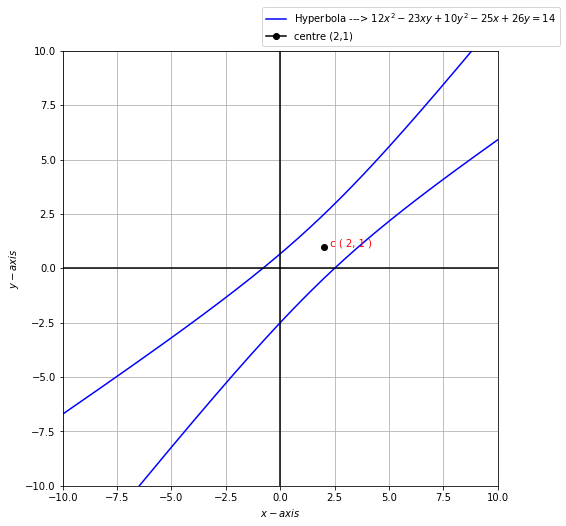
\includegraphics[width=\columnwidth]{./solutions/40/1/Assignment 8.png}
    \caption{Hyperbola when origin is shifted}
    \label{eq:solutions/40/1/Fig :1}
\end{figure}

The figure \ref{eq:solutions/40/1/Fig :1} verifies the given equation \eqref{eq:solutions/40/1/given} as hyperbola with centre $\myvec{2\\1}$



\item What conic does the following equation represent. 
\begin{align}
13x^2-18xy+37y^2+2x+14y-2 = 0
\end{align}
Find the center.
\\
\solution
The general second degree equation can be expressed as follows,
\begin{align}
\vec{x^T}\vec{V}\vec{x}+2\vec{u^T}\vec{x}+f=0\label{eq:solutions/15/40/2/eqmain}
\end{align}
From the given second degree equation we get,
\begin{align}
\vec{V} &= \myvec{13&-9\\-9&37}\\
\vec{u} &= \myvec{1\\7}\\
f &= -2
\end{align}
Expanding the determinant of $\vec{V}$ we observe, 
\begin{align}
\mydet{13&-9\\-9&37} = 400>0 \label{eq:solutions/15/40/2/eqV}
\end{align}
Hence from \eqref{eq:solutions/15/40/2/eqV} we conclude that given equation is an ellipse. The characteristic equation of $\vec{V}$ is given as follows,
\begin{align}
\mydet{\lambda\vec{I}-\vec{V}} = \mydet{\lambda-13&9\\9&\lambda-37} &= 0\\
\implies \lambda^2-50\lambda+400 &= 0\label{eq:solutions/15/40/2/eqchar}
\end{align}
Hence the characteristic equation of $\vec{V}$ is given by \eqref{eq:solutions/15/40/2/eqchar}. The roots of \eqref{eq:solutions/15/40/2/eqchar} i.e the eigenvalues are given by
\begin{align}
\lambda_1=10, \lambda_2=40\label{eq:solutions/15/40/2/eqeigenvals}    
\end{align}
The eigen vector $\vec{p}$ is defined as, 
\begin{align}
\vec{V}\vec{p} &= \lambda\vec{p}\\
\implies\brak{\lambda\vec{I}-\vec{V}}\vec{p}&=0
\end{align}
for $\lambda_1=10$,
\begin{align}
\brak{\lambda_1\vec{I}-\vec{V}}&=\myvec{-3&9\\9&-27}\xleftrightarrow[R_1=\frac{1}{3}R_1]{R_2=R_2+3R_1}\myvec{-1&3\\0&0}\\
\implies\vec{p_1}&=\myvec{3\\1}
\end{align}
Again, for $\lambda_2=40$,
\begin{align}
\brak{\lambda_2\vec{I}-\vec{V}}&=\myvec{27&9\\9&3}\xleftrightarrow[R_1=\frac{1}{27}R_1]{R_2=R_2-R_1}\myvec{1&\frac{1}{3}\\0&0}\\
\implies\vec{p_2}=\myvec{-1\\3}
\end{align}
Again, 
Hence from the equation
\begin{align}
\vec{V}&=\vec{P}\vec{D}\vec{P^{-1}}
%\intertext{Where $\vec{D}$ is a diagonal matrix, we get,}
\vec{P}&=\myvec{\vec{p_1}&\vec{p_2}}=\myvec{3&-1\\1&3}\\
\vec{D}&=\myvec{10&0\\0&40}
\end{align}
Now \eqref{eq:solutions/15/40/2/eqmain} can be written as,
\begin{align}
\vec{y^T}\vec{D}\vec{y}&=\vec{u^T}\vec{V^{-1}}\vec{u}-f\qquad\text{$\mydet{\vec{V}}\not=0$}\label{eq:solutions/15/40/2/eqnewmain}\\
\intertext{And,}
\vec{c}&= -\vec{V^{-1}}\vec{u}\qquad\text{$\mydet{\vec{V}}\not=0$}\label{eq:solutions/15/40/2/eqcenter}\\
\vec{y} &= \vec{P^T}\brak{\vec{x-c}}\label{eq:solutions/15/40/2/eqY}
\end{align}
The centre/vertex of the conic section in \eqref{eq:solutions/15/40/2/eqmain} is given by $\vec{c}$ in \eqref{eq:solutions/15/40/2/eqcenter}. 
We compute $\vec{V^{-1}}$ as follows,
\begin{align}
\myvec{13&-9&1&0\\-9&37&0&1}&\xleftrightarrow[R_2=\frac{13}{400}R_2]{R_2=R_2+\frac{9}{13}R_1}\myvec{13&-9&1&0\\0&1&\frac{9}{400}&\frac{13}{400}}\\
&\xleftrightarrow[R_1=R_1+\frac{9}{13}R_2]{R_1=\frac{1}{13}R_1}\myvec{1&0&\frac{37}{400}&\frac{9}{400}\\0&1&\frac{9}{400}&\frac{13}{400}}
\end{align}
Hence $\vec{V^{-1}}$ is given by,
\begin{align}
\vec{V^{-1}} = \myvec{\frac{37}{400}&\frac{9}{400}\\\frac{9}{400}&\frac{13}{400}}
\end{align}
Now $\vec{u^T}\vec{V^{-1}}\vec{u}$ is given by,
\begin{align}
\vec{u^T}\vec{V^{-1}}\vec{u}&=\frac{1}{400}\myvec{1&7}\myvec{37&9\\9&13}\myvec{1\\7}=2\label{eq:solutions/15/40/2/eqRHS}\\
\intertext{And, $\vec{V^{-1}}\vec{u}$ is given by,}
\vec{V^{-1}}\vec{u} &= \frac{1}{400}\myvec{100\\100}=\frac{1}{4}\myvec{1\\1}\label{eq:solutions/15/40/2/eqcenterRHS}
\end{align}
By putting the value of \eqref{eq:solutions/15/40/2/eqcenterRHS}, the center of the ellipse is given by \eqref{eq:solutions/15/40/2/eqcenter} as follows,
\begin{align}
\vec{c} = -\frac{1}{4}\myvec{1\\1} = \myvec{-\frac{1}{4}\\-\frac{1}{4}}
\end{align}
Also the semi-major axis ($a$) and semi-minor axis ($b$) of the ellipse are given by,
\begin{align}
a = \sqrt{\frac{\vec{u^T}\vec{V^{-1}}\vec{u}-f}{\lambda_1}}=\frac{\sqrt{10}}{5}\\
b = \sqrt{\frac{\vec{u^T}\vec{V^{-1}}\vec{u}-f}{\lambda_2}}=\frac{\sqrt{10}}{10}
\end{align}
Finally from \eqref{eq:solutions/15/40/2/eqnewmain}, the equation of ellipse is given by,
\begin{align}
&\vec{y^T}\myvec{10&0\\0&40}\vec{y}=4\label{eq:solutions/15/40/2/eqFinal}
\end{align}

The following figure \ref{eq:solutions/15/40/2/fig:my_label}
is the graphical representation of the ellipse in \eqref{eq:solutions/15/40/2/eqFinal},
\begin{figure}[t]
\centering
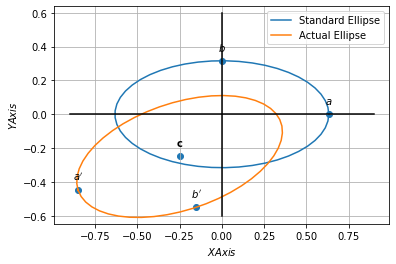
\includegraphics[width = \columnwidth]{./solutions/40/2/Ellipse.png}
\caption{Graphical representation of the ellipse}
\label{eq:solutions/15/40/2/fig:my_label}
\end{figure}


%
\item What conic does the following equation represent?
\begin{align}
y^2-2\sqrt{3}xy+3x^2+6x-4y+5 = 0
\end{align}
Find the center.
\\
\solution
The general second degree equation can be expressed as follows,
\begin{align}
\vec{x^T}\vec{V}\vec{x}+2\vec{u^T}\vec{x}+f=0\label{eq:solutions/40/3/eqmain}
\end{align}
From the given second degree equation we get,
\begin{align}
\vec{V} &= \myvec{3&-\sqrt{3}\\-\sqrt{3}&1}\\ \label{eq:solutions/40/3/given1}
\vec{u} &= \myvec{3\\-2}\\ 
f &= 5 \label{eq:solutions/40/3/given2}
\end{align}
Expanding the determinant of $\vec{V}$ we observe, 
\begin{align}
\mydet{3&-\sqrt{3}\\-\sqrt{3}&1} = 0 \label{eq:solutions/40/3/eq2.1}
\end{align}
Also
\begin{align}
    \mydet{\vec{V}&\vec{u} \\\vec{u}^T & f}=
    \mydet{3&-\sqrt{3}&3\\-\sqrt{3}&1 &-2\\3 &-2&5}
    \neq 0\label{eq:solutions/40/3/eq2.2}\end{align}
Hence from \eqref{eq:solutions/40/3/eq2.1} and \eqref{eq:solutions/40/3/eq2.2} we conclude that given equation is a parabola. The characteristic equation of $\vec{V}$ is given as follows,
\begin{align}
\mydet{\vec{V}-\lambda\vec{I}} = \mydet{3-\lambda &-\sqrt{3}\\-\sqrt{3}& 1-\lambda} &= 0\\
\implies \lambda^2-4\lambda &= 0\label{eq:solutions/40/3/eqchar}
\end{align}
Hence the characteristic equation of $\vec{V}$ is given by \eqref{eq:solutions/40/3/eqchar}. The roots of \eqref{eq:solutions/40/3/eqchar} i.e the eigenvalues are given by
\begin{align}
\lambda_1=0, \lambda_2=4\label{eq:solutions/40/3/eqeigenvals}    
\end{align}
The eigen vector $\vec{p}$ is defined as, 
\begin{align}
\vec{V}\vec{p} &= \lambda\vec{p}\\
\implies\brak{\vec{V}-\lambda\vec{I}}\vec{p}&=0 \label{eq:solutions/40/3/eqev}
\end{align}
for $\lambda_1=0$,
\begin{align}
\brak{\vec{V}-\lambda_1\vec{I}}&=\myvec{3&-\sqrt{3}\\-\sqrt{3}&1}\xleftrightarrow[R_1=\frac{1}{\sqrt{3}}R_1]{R_2=R_1+R_2}\myvec{\sqrt{3}&-1\\0&0}\label{eq:solutions/40/3/eq2.3.0}
\end{align}
Substiuting equation \ref{eq:solutions/40/3/eq2.3.0} in equation \ref{eq:solutions/40/3/eqev} and upon normalizing we get we get
\begin{align}
\implies\vec{p_1}&=\myvec{1/2\\\sqrt{3}/2} \label{eq:solutions/40/3/eq2.3}
\end{align}
Again, for $\lambda_2=4$,
\begin{align}
\brak{\vec{V}-\lambda_2\vec{I}}&=\myvec{-1&-\sqrt{3}\\-\sqrt{3}&-3}\xleftrightarrow[R_1=-\sqrt{3}R_1]{R_2=-\sqrt{3}R_1+R_2}\myvec{1&\sqrt{3}\\0&0} \label{eq:solutions/40/3/eq2.3.1}
\end{align}
Substiuting equation \ref{eq:solutions/40/3/eq2.3.1} in equation  \ref{eq:solutions/40/3/eqev} and upon normalizing we get
\begin{align}
        \vec{p_2}&=\myvec{-\sqrt{3}/2 \\1/2} \label{eq:solutions/40/3/eqp1}
\end{align}
The matrix $\vec{P}$,
\begin{align}
\vec{P}&=\myvec{\vec{p_1}&\vec{p_2}}=\myvec{1/2&-\sqrt{3}/2\\\sqrt{3}/2&1/2} \\
\vec{D}&=\myvec{0&0\\0&4}
\end{align}
\begin{align}
    \eta=2\vec{p_1}^T\vec{u}=3-2\sqrt{3} 
\end{align}
The focal length of the parabola is given by:
\begin{align}
    \abs{\frac{\eta}{\lambda_2}} 
    = \abs{\frac{3-2\sqrt{3}}{4}} = 0.116
\end{align}
When $\mydet{\vec{V}}=0$, \eqref{eq:solutions/40/3/eqmain} can be written as
\begin{align}
    \vec{y^T}\vec{D}\vec{y}&=-\eta\myvec{1&0}\vec{y}\label{eq:solutions/40/3/eq2.4}
    \intertext{And the vertex $\vec{c}$ is given by }
    \myvec{\vec{u^T}+\frac{\eta}{2}\vec{p_1^T} \\ \vec{V}}\vec{c}=
    \myvec{-f \\ \frac{\eta}{2}\vec{p_1}-\vec{u}}\label{eq:solutions/40/3/eqa} 
\end{align}
Substituting the found values
\begin{align}
\vec{u}^T + \frac{\eta}{2}\vec{p_1}^T = \myvec{3&-2}+\frac{3-2\sqrt{3}}{2}\myvec{\frac{1}{2}&\frac{\sqrt{3}}{2}}\\
\implies\vec{u}^T + \frac{\eta}{2}\vec{p_1}^T =\myvec{\frac{15-2\sqrt{3}}{4}&\frac{-14+3\sqrt{3}}{4}}\label{eq:solutions/40/3/eq2.23} \\
\frac{\eta}{2} \vec{p_1} -\vec{u}= \myvec{\frac{-9-2\sqrt{3}}{4}\\ \frac{2+3\sqrt{3}}{4}}\label{eq:solutions/40/3/eq2.24}
\end{align}
using equations \eqref{eq:solutions/40/3/given1},\eqref{eq:solutions/40/3/given2},\eqref{eq:solutions/40/3/eq2.3},\eqref{eq:solutions/40/3/eq2.23},\eqref{eq:solutions/40/3/eq2.24} and \eqref{eq:solutions/40/3/eq2.3} in \eqref{eq:solutions/40/3/eqa}
\begin{align}
    \myvec{\frac{15-2\sqrt{3}}{4}&\frac{-14+3\sqrt{3}}{4}\\3 & -\sqrt{3}\\ -\sqrt{3}& 1}\vec{c} =\myvec{ -5\\\frac{-9-2\sqrt{3}}{4}\\ \frac{2+3\sqrt{3}}{4}}\label{eq:solutions/40/3/eqcen}
\end{align}
By performing row reductions on augmented matrix
\begin{multline}
\myvec{\frac{15-2\sqrt{3}}{4}&\frac{-14+3\sqrt{3}}{4}&-5\\3 & -\sqrt{3}&\frac{(-9-2\sqrt{3})}{4}\\ -\sqrt{3}& 1&\frac{2+3\sqrt{3}}{4}}{R_2\xleftrightarrow[]{}{R_1}}\\
\myvec{3 & -\sqrt{3}&\frac{(-9-2\sqrt{3})}{4}\\\frac{15-2\sqrt{3}}{4}&\frac{-14+3\sqrt{3}}{4}&-5\\-\sqrt{3}& 1&\frac{2+3\sqrt{3}}{4} }
\end{multline}
\begin{multline}
\myvec{3 & -\sqrt{3}&\frac{(-9-2\sqrt{3})}{4}\\\frac{15-2\sqrt{3}}{4}&\frac{-14+3\sqrt{3}}{4}&-5\\-\sqrt{3}& 1&\frac{2+3\sqrt{3}}{4}}
\xleftrightarrow[]{R_2\leftarrow R_2-\frac{15-2\sqrt{3}}{12}R_1}\\
\myvec{3 & -\sqrt{3}&\frac{(-9-2\sqrt{3})}{4}\\0 & 2(\sqrt{3}-2) & \frac{(4\sqrt{3}-39)}{16}\\\sqrt{3}& 1&\frac{2+3\sqrt{3}}{4}}
\end{multline}
Therefore, 
\begin{multline}
 \myvec{3 & -\sqrt{3}&\frac{(-9-2\sqrt{3})}{4}\\0&2(\sqrt{3}-2)&\frac{(4\sqrt{3}-39)}{16}\\-\sqrt{3}& 1&\frac{(2+3\sqrt{3})}{4}}\xleftrightarrow[]{R_3\leftarrow R_3+\frac{1}{\sqrt{3}}R_1}\\
\myvec{3 & -\frac{433}{250}&-\frac{311}{100}\\0 & -\frac{107}{200} & -2\\0& 0&0}
\end{multline}
\begin{figure}[!h]
    \centering
    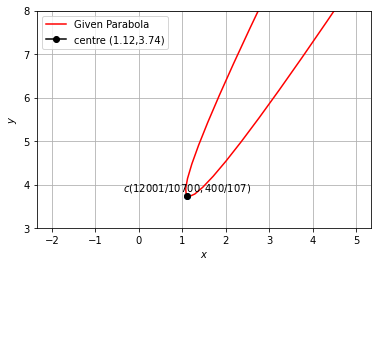
\includegraphics[width=\columnwidth]{./solutions/40/3/parabola.png}
    \caption{Parabola with the center c}
    \label{eq:solutions/40/3/Fig:1}
\end{figure}
\begin{multline}
\myvec{3 & -\frac{433}{250}&-\frac{311}{100}\\0 & -\frac{107}{200} & -2\\0& 0&0}\xleftrightarrow[]{R_1\leftarrow \frac{R_1}{{3}}}\\\myvec{1& -\frac{433}{750}&-\frac{311}{300}\\0 & -\frac{107}{200} & -2\\0& 0&0}
\end{multline}
\begin{multline}
\myvec{1 & -\frac{433}{750}&-\frac{311}{300}\\0 & -\frac{107}{200} & -2\\0& 0&0}\xleftrightarrow[]{R_2\leftarrow \frac{-200}{{107}}R_2}\\
\myvec{1 & -\frac{433}{750}&-\frac{311}{300}\\0 & 1 & \frac{400}{107}\\0& 0&0}
\end{multline}

\begin{multline}
\myvec{1 & -\frac{433}{750}&-\frac{311}{300}\\0 & 1 & \frac{400}{107}\\0& 0&0}\xleftrightarrow[]{R_1\leftarrow R_1+\frac{433}{{750}}R_2}\\
\myvec{1 & 0&\frac{12001}{10700}\\0 & 1 & \frac{400}{107}\\0& 0&0}\label{eq:solutions/40/3/eq7}
\end{multline}
On solving for values of $\vec{c}$ from \eqref{eq:solutions/40/3/eq7} 
 The vertex of parabola is $\vec{c}$=$\myvec{\frac{12001}{10700}\\\frac{400}{107}}$.
 

\item What conics do the following equation represent? When possible, find the centres and also their equations referred to the centre.
\begin{align}
2x^2-72xy+23y^2-4x-2y-48=0\label{eq:solutions/40/4/ques}
\end{align}
\solution
%
The second degree equation in general can be represented as
\begin{align}
    ax^2+2bxy+cy^2+2dx+2ey+f=0\label{eq:solutions/40/4/general}
\end{align}
The equation \eqref{eq:solutions/40/4/general} in matrix form can be represented as 
\begin{align}
%&\vec{x}^T\myvec{12 & \frac{-23}{2}\\\frac{-23}{2} & %10}\vec{x}+2\myvec{\frac{-25}{2} & 13}\vec{x}-14=0\label{eq:solutions/40/4/given}
\vec{x}^T\vec{V}\vec{x}+2\vec{u}^T\vec{x}+f=0\label{eq:solutions/40/4/given}
\end{align}
where 
\begin{align}
\vec{V}=\myvec{a&b\\b&c}=\myvec{2 & -36\\-36 & 23}\\
\vec{u}=\myvec{d\\e}=\myvec{-2 \\ -1}\\
f=-48
\end{align}
\begin{align}
    \det(\vec{V})=\begin{array}{|cc|} 2 & -36\\-36 & 23 \end{array}\\
\implies\det(\vec{V})=-1250\\
\implies\det(\vec{V})<0
\end{align}
Since $\det(\vec{V})<0$ the given equation \eqref{eq:solutions/40/4/ques} represents a hyperbola. The characteristic equation of $\vec{V}$ is acquired by evaluating the determinant 
\begin{align}
       \begin{array}{|c|}
V-\lambda\vec{I}
\end{array}=0\\
   \begin{array}{|cc|}
2-\lambda & -36 \\ -36 & 23-\lambda
\end{array}=0\\
\implies \lambda^2-25\lambda-1250=0\label{eq:solutions/40/4/eqroots}
\end{align}
On solving the equation \eqref{eq:solutions/40/4/eqroots}, the eigen values are given by 
\begin{align}
    \lambda_1=50\label{eq:solutions/40/4/eqeig1}\\
    \lambda_2=-25\label{eq:solutions/40/4/eqeig2}
\end{align}
We can observe that for a hyperbola, $\lambda_1>0$ and  $\lambda_2<0$.
Consider the eigenvector $\vec{p}=\myvec{v_1\\v_2}$ is defined as 
\begin{align}
    \vec{V}\vec{p}&=\lambda\vec{p}\\
    \implies (\vec{V}-\lambda\vec{I})\vec{p}&=0\label{eq:solutions/40/4/cheq}
\end{align}
For $\lambda_1=50$ ,
\begin{align}
    (\vec{V}-\lambda_1\vec{I})=\myvec{-48&-36\\-36&-27}
\end{align}
By row reduction , 
\begin{align}
    \myvec{-48&-36\\-36&-27}\\
    \xleftrightarrow[R_1\leftarrow\frac{R_1}{-12}]{R_2\leftarrow\frac{R_2}{-9}}\myvec{4&3\\4&3}\\
    \xleftrightarrow[]{R_2\leftarrow R_2-R_1}
    \myvec{4&3\\0&0}\label{eq:solutions/40/4/ref1}
\end{align}
Subsituting equation \eqref{eq:solutions/40/4/ref1} in equation \eqref{eq:solutions/40/4/cheq} we get
\begin{align}
        \myvec{4&3\\0&0}\myvec{v_1\\v_2}=\myvec{0\\0}\label{eq:solutions/40/4/eig1}
\end{align}
Eigen vector $\vec{p_1}$ is given by
\begin{align}
    \vec{p_1}=\myvec{\frac{-3}{4}\\1}\label{eq:solutions/40/4/ev1}
\end{align}
For $\lambda_2=-25$ ,
\begin{align}
    (\vec{V}-\lambda_2\vec{I})=\myvec{27&-36\\-36&48}
\end{align}
By row reduction , 
\begin{align}
    \myvec{27&-36\\-36&48}\\
    \xleftrightarrow[R_1\leftarrow\frac{R_1}{9}]
    {R_2\leftarrow\frac{R_2}{-12}}
    \myvec{3&-4\\3&-4}\\
    \xleftrightarrow[]{R_2\leftarrow R_2-R_1}
    \myvec{3&-4\\0&0}\label{eq:solutions/40/4/ref2}
\end{align} 
Subsituting equation \eqref{eq:solutions/40/4/ref2} in equation \eqref{eq:solutions/40/4/cheq} we get 
\begin{align}
    \myvec{3&-4\\0&0}\myvec{v_1\\v_2}=\myvec{0\\0}\label{eq:solutions/40/4/eig2}
\end{align}
Eigen vector $\vec{p_2}$ is given by
\begin{align}
        \vec{p_2}=\myvec{\frac{4}{3}\\1}\label{eq:solutions/40/4/ev2}
\end{align}
By eigen decompostion, $\vec{V}$ can be represented by
\begin{align}
    \vec{V}=\vec{P}\vec{D}\vec{P}^T\label{eq:solutions/40/4/evd}
\end{align}
where 
\begin{align}
        \vec{P}=\myvec{\vec{p_1} & \vec{p_2}}\label{eq:solutions/40/4/eqp}\\
    \vec{D}=\myvec{\lambda_1 & 0 \\0 & \lambda_2}\label{eq:solutions/40/4/eqD}
\end{align}
Substituting equations \eqref{eq:solutions/40/4/ev1}, \eqref{eq:solutions/40/4/ev2} in equation \eqref{eq:solutions/40/4/eqp} we get 
\begin{align}
    \vec{P}=\myvec{\frac{-3}{4}&\frac{4}{3}\\1&1}\label{eq:solutions/40/4/eqP}
\end{align}
Substituting equations \eqref{eq:solutions/40/4/eqeig1}, \eqref{eq:solutions/40/4/eqeig2} in \eqref{eq:solutions/40/4/eqD} we get
\begin{align}
       \vec{D}=\myvec{50 & 0\\0 & -25}\label{eq:solutions/40/4/eqDD}
\end{align}
Centre of the hyperbola is given by 
\begin{align}
    \vec{c}=-\vec{V}^{-1}\vec{u}
\end{align}
\begin{align}
    \implies\vec{c}=-\myvec{\frac{-23}{1250}&\frac{-18}{625}\\\frac{-18}{625}&\frac{-1}{625}}\myvec{-2\\-1}\\
    \implies\vec{c}=\myvec{\frac{-41}{625}\\\frac{-37}{625}}
\end{align}
Since,
\begin{align}
    \vec{u}^T\vec{V}^{-1}\vec{u}-f = \frac{-30119}{625}<0\label{eq:solutions/40/4/cond}
\end{align} 
We swap the semi-major and semi-minor axes and the respective are given by
\begin{align}
axes=
\begin{cases}
\sqrt{\frac{\vec{u}^T\vec{V}^{-1}\vec{u}-f}{\lambda_2}}\\ \sqrt{\frac{f-\vec{u}^T\vec{V}^{-1}\vec{u}}{\lambda_1}}
\end{cases}
\end{align}
Calculating the axes, we get
\begin{align}
\sqrt{\frac{\vec{u}^T\vec{V}^{-1}\vec{u}-f}{\lambda_2}}=1.388\\
\sqrt{\frac{f-\vec{u}^T\vec{V}^{-1}\vec{u}}{\lambda_1}}=0.981
\end{align}
The figure \ref{eq:solutions/40/4/Fig :1} verifies the given equation \eqref{eq:solutions/40/4/given} as hyperbola with centre $\myvec{\frac{-41}{625}\\\frac{-37}{625}}$
\begin{figure}[h]
    \centering
    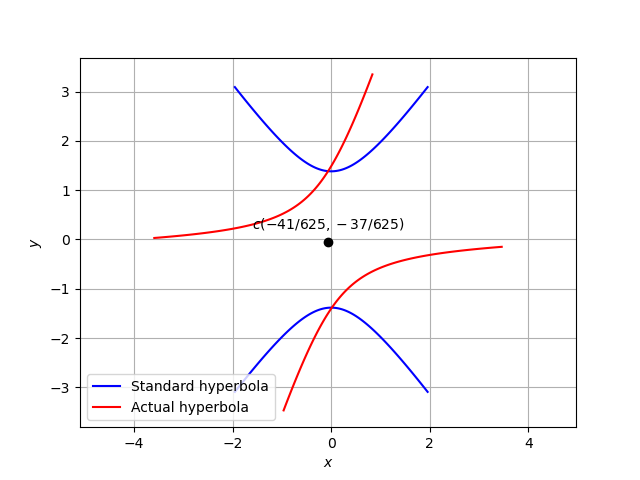
\includegraphics[width=\columnwidth]{./solutions/40/4/Hyperbola.png}
    \caption{Hyperbola when origin is shifted}
    \label{eq:solutions/40/4/Fig :1}
\end{figure}
\item  Now \eqref{eq:solutions/40/4/given} can be written as,
\begin{align}
    \vec{y}^T\vec{D}\vec{y}=\vec{u}^T\vec{V}^{-1}\vec{u}-f\label{eq:solutions/40/4/fi}
\end{align}
where ,
\begin{align}
    \vec{y}&=\vec{P}^T(\vec{x}-\vec{c})
\end{align}
To get $\vec{y}$,
\begin{align}
    \vec{y}=\vec{P}^T\vec{x}-\vec{P}^T\vec{c}\\
    \vec{y}=\myvec{\frac{-3}{4}&1\\\frac{4}{3}&1}\vec{x}-
    \myvec{\frac{-3}{4}&1\\\frac{4}{3}&1}\myvec{\frac{-41}{625}\\\frac{-37}{625}}\\
    \vec{y}=\myvec{\frac{-3}{4}&1\\\frac{4}{3}&1}\vec{x}-
    \myvec{\frac{-1}{100}\\\frac{-11}{75}}
\end{align}
Subsituting the eqauations \eqref{eq:solutions/40/4/cond}, \eqref{eq:solutions/40/4/eqDD} in equation \eqref{eq:solutions/40/4/fi}
\begin{align}
    \vec{y}^T\myvec{50&0\\0&-25}\vec{y}=\frac{-30119}{625}
\end{align}

\item What conic does the given equations represent?
\begin{align}
6x^2-5xy-6y^2+14x+5y+4=0
\end{align}
\\
\solution
The above equation can be expressed in the form 
\begin{align}
\vec{x}^T\vec{V}\vec{x}+2\vec{u}^T\vec{x}+f&=0 \label{eq:solutions/40/5/eq1}
\intertext{Comparing equation we get}
    \vec{V}=\vec{V}^T&=\myvec{6 & \frac{-5}{2}\\\frac{-5}{2} &-6}\label{eq:solutions/40/5/eqv}\\
    \vec{u}&=\myvec{7 \\ \frac{5}{2}}\label{eq:solutions/40/5/equ}\\
    f&=4\label{eq:solutions/40/5/eqfv}
\end{align}    
The above equation \eqref{eq:solutions/40/5/eq1} represents a pair of straight lines if
\begin{align}
    \begin{array}{|cc|}
\vec{V} & \vec{u}\\\vec{u}^T & f
\end{array}&=0\label{eq:solutions/40/5/eqcheck}
\end{align}
Verify the given equation as if it is pair of straight lines
\begin{align}
\Delta&=\begin{array}{|ccc|}
6 &\frac{-5}{2}& 7\\\frac{-5}{2} & -6 & \frac{5}{2}\\ 7 & \frac{5}{2} & 4
\end{array}\\
\implies \ 6\mydet{-6 & \frac{5}{2} \\ \frac{5}{2} & 4} 
		& -\frac{-5}{2}\mydet{-\frac{5}{2} & \frac{5}{2} \\ 7 & 4}
		+7\mydet{-\frac{5}{2} & -6 \\ 7 & \frac{5}{2}} = 0 \label{eq:solutions/40/5/eq10}\\
\implies \Delta&=0
\end{align}
Since equation \eqref{eq:solutions/40/5/eqcheck} is satisfied, we could say that the given equation represents two straight lines
\begin{align}
    \Delta_{V} &= \begin{array}{|cc|}
6 &\frac{-5}{2}\\\frac{-5}{2} & -6
\end{array}<0
\end{align}
Let the equations of lines be,
\begin{align}
	\brak{\vec{n_1}^T \vec{x} - c_1}\brak{\vec{n_1}^T \vec{x} - c_1} =
        \vec{x}^{T}\vec{Vx} + 2\vec{u}^{T}\vec{x} + f=0\label{eq:solutions/40/5/eq:eql03}
\end{align}
\begin{align}
\brak{\vec{n_1}^T\vec{x}-c_1}\brak{\vec{n_2}^T\vec{x}-c_2}
&=\vec{x}^T\myvec{6 & \frac{-5}{2} \\\frac{-5}{2} & -6}\vec{x}\notag\\
+2\myvec{7 & \frac{5}{2}}\vec{x}+4\label{eq:solutions/40/5/equate}\\
    \vec{n_1}*\vec{n_2} = \myvec{a\\2b\\c} &= \myvec{6\\-5\\-6}\label{eq:solutions/40/5/conv}\\
    c_2\vec{n_1}+c_1\vec{n_2}&=-2\myvec{7\\\frac{5}{2}}\label{eq:solutions/40/5/eqc1c2}\\
    c_1c_2&=4
\end{align}
The slopes of the lines are given by the roots of the polynomial 
\begin{align}
    &cm^2+2bm+a=0\label{eq:solutions/40/5/e}\\
    \implies m_i&=\frac{-b\pm{\sqrt{-\Delta_{V}}}}{c}\\
    \vec{n_i}&=k\myvec{-m_i\\1}
\end{align}
Substituting the given data in above equations \eqref{eq:solutions/40/5/e} we get,
\begin{align}
    &-6m^2-5m+6=0\\
    &\implies m_i=\frac{\frac{-5}{2}\pm{\sqrt{-(\frac{-169}{4})}}}{-6}\label{eq:solutions/40/5/m}
\intertext{Solving equation \eqref{eq:solutions/40/5/m} we get,}
    m_1&=-\frac{3}{2},  m_2=\frac{2}{3}\\
   % \vec{m_1}=\myvec{-2\\3}, \vec{m_2}=\myvec{3\\ 2}\\
   &= \vec{n_1}=\myvec{-3\\ -2}, \vec{n_2}=\myvec{-2\\3} \label{eq:solutions/40/5/eq:normal1}
\intertext{We know that,}
\vec{n_1}\ast \vec{n_2} = \myvec{a\\2b\\c} \label{eq:solutions/40/5/eq:conv1}
\end{align}
Verification using Toeplitz matrix, From equation \eqref{eq:solutions/40/5/eq:normal1}
\begin{align}
    \vec{n_1}=\myvec{-3&0\\-2&-3\\0&-2}
    \vec{n_2}=\myvec{-2\\3}\label{eq:solutions/40/5/eq:conv2}\\
\implies \myvec{-3&0\\-2&-3\\0&-2}\myvec{-2\\ 3} = \myvec{6\\-5\\-6} = \myvec{a\\2b\\c}\label{eq:solutions/40/5/eq:conv3}
\end{align}
$\implies$ Equation \eqref{eq:solutions/40/5/eq:normal1} satisfies \eqref{eq:solutions/40/5/eq:conv1}\\
$c_1$ and $c_2$ can be obtained as,
\begin{align}
\myvec{\vec{n_1} & \vec{n_2}}\myvec{c_2\\c_1}&=-2\vec{u} \label{eq:solutions/40/5/eq:aug1}
\end{align}
Substituting \eqref{eq:solutions/40/5/eq:normal1} in \eqref{eq:solutions/40/5/eq:aug1}, the augmented matrix is,
\begin{align}
\myvec{-3 & -2 & 14 \\ -2 & 3 & 5}
\xleftrightarrow[R_2\leftarrow R_2+2R_1]{R_1\leftarrow -R_1/3}
\myvec{1 &\frac{2}{3} &-\frac{14}{3} \\ 0& \frac{13}{3} & -\frac{13}{3}} \label{eq:solutions/40/5/eq:aug5}\\
\xleftrightarrow[R_1\leftarrow R_1-\frac{2}{3}R_2]{R_2\leftarrow \frac{3}{13}R_2}
\myvec{1 &0 &-4 \\ 0& 1 & -1} \label{eq:solutions/40/5/eq:aug2}\\
\implies c_1 = -4, c_2=-1 \label{eq:solutions/40/5/eq:const1}
\end{align}
Equations \eqref{eq:solutions/40/5/eq:eql03}, can be modified as,from \eqref{eq:solutions/40/5/eq:normal1} and \eqref{eq:solutions/40/5/eq:const1} in we get,
\begin{align}
    \myvec{-3 & -2}\vec{x}&=-4\\
    \myvec{-2 & 3}\vec{x}&=-1
\end{align}
\begin{multline}
\implies \brak{-3x-2y+4}\brak{-2x+3y+1}= 0\\
\implies \boxed{\brak{3x+2y-4}\brak{2x-3y-1} = 0} \label{eq:solutions/40/5/eq:line1}
\end{multline}
The angle between the lines can be expressed as, 
\begin{align}
	\vec{n_1}=\myvec{-3\\-2} , \quad \vec{n_2}=\myvec{-2\\3}\\
	\cos\theta=\frac{\vec{n_1}^T\vec{n_2}}{\norm{\vec{n_1}}\norm{\vec{n_2}}} \\
	\implies \quad \theta=\cos^{-1}({\frac{0}{\sqrt{169}}}) = 90\degree.
\end{align}
\begin{figure}[h]
    \centering
    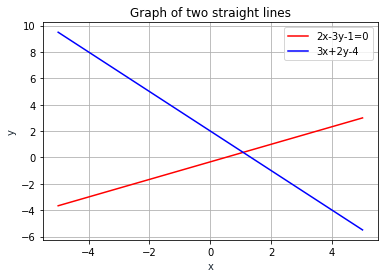
\includegraphics[width=\columnwidth]{./solutions/40/5/A6.png}
    \caption{Pair of straight lines}
    \label{eq:solutions/40/5/Fig :1}
\end{figure}

\item What conic does the following equation represent? Find its equation and centre.
\begin{align*}
	3x^2 - 8xy - 3y^2 + 10x - 13y + 8 =0 
\end{align*}
\solution
The general equation of second degree can be expressed as
\begin{align}
	\vec{x}^{T}\vec{Vx} + 2\vec{u}^{T}\vec{x} + f=0   \label{eq:solutions/40/6/stdsecdeg}
\end{align}
where
\begin{align}
        \vec{V}=\vec{V}^T=\myvec{a & b \\ b & c}   \label{eq:solutions/40/6/V}  \\
        \vec{u}^T=\myvec{d &  e}            \label{eq:solutions/40/6/u}
\end{align}
From (\ref{eq:solutions/40/6/V}) and (\ref{eq:solutions/40/6/u})
\begin{align}
	\vec{V}=\vec{V}^T &= \myvec{3 & -4 \\ -4 & -3} \\
	\vec{u} &= \myvec{5 \\ -\frac{13}{2}}
\end{align}
\begin{align}
	\mydet{\vec{V}}=\mydet{3 & -4 \\ -4 & 3} =-25 \\
	\implies \mydet{\vec{V}} < 0       \label{eq:solutions/40/6/detless0}
\end{align}
Since $ \vec{V} = \vec{V}^T $, there exists an orthogonal matrix $\vec{P}$ such that
\begin{align}
	\vec{P}\vec{V}\vec{P}^T = \vec{D} = diag\myvec{\lambda_1 & \lambda_2}
\end{align}
or equivalently 
\begin{align}
	\vec{V} = \vec{P}\vec{D}\vec{P}^T
\end{align}
Eigen vectors of real symmetric matrix $\vec{V}$ are orthogonal. The characteristic equation of $\vec{V}$ is obtained by evaluating the determinant
\begin{align}
	\mydet{\lambda\vec{I}-\vec{V}} = \mydet{\lambda-3 & 4 \\ 4 & \lambda + 3} = 0 \\
	\implies \quad \lambda^2-25=0 \\
	\implies \quad \lambda_1=-5,\lambda_2=5   \label{eq:solutions/40/6/lambdavals}
\end{align}
From (\ref{eq:solutions/40/6/detless0}) and (\ref{eq:solutions/40/6/lambdavals}) the equation represents a hyperbola.
The eigen vector $\vec{p}$ is defined as
\begin{align}
	\vec{V}\vec{p}=\lambda\vec{p} \\
	\implies (\lambda\vec{I} - \vec{V})\vec{p}=0
\end{align}
For $\lambda_1 = -5$ :
\begin{align}
	(\lambda_1\vec{I}-\vec{V})=\myvec{-8 & 4 \\ 4 & -2} 
	\xleftrightarrow[R_2 \leftarrow \frac{R_2}{2}]{R_1 \leftarrow -\frac{R_1}{4}}
	\myvec{2 & -1 \\ 2 & -1} \\
	\xleftrightarrow[]{R_2 \leftarrow R_2 - R_1}
	\myvec{2 & -1 \\ 0 & 0} \\
	\implies \vec{p_1}=\frac{1}{\sqrt{5}}\myvec{2 \\ 1}
\end{align}
Similarly, the eigenvector corresponding to $\lambda_2$ can be obtained as
\begin{align}
	\vec{p_2}=\frac{1}{\sqrt{5}}\myvec{-1\\2}
\end{align}
The orthogonal eigen-vector matrix
\begin{align}
	\vec{P}=\myvec{\vec{p_1} & \vec{p_2}}
	=\frac{1}{\sqrt{5}}\myvec{2 & -1 \\ 1 & 2} \\
	\vec{D}=\myvec{-5 & 0 \\ 0 & 5}
\end{align}
Let $\vec{x}=\vec{P}\vec{y} + \vec{c} $ with $\vec{c}=-\vec{V}^{-1}\vec{u}$. Substituting in (\ref{eq:solutions/40/6/stdsecdeg})
\begin{align}
	\vec{y}^T\vec{D}\vec{y}=\vec{u}^T\vec{V}^{-1}\vec{u}-f 
\end{align}
with centre
\begin{align}
	\vec{c}=-\vec{V^{-1}u}=\myvec{-\frac{41}{25} \\ \frac{1}{50}} 
\end{align}
and minor and major axes parameters as
\begin{align}
	\sqrt{\frac{\lambda_1}{f-\vec{u^{T}V^{-1}u}}} = \sqrt{\frac{500}{33}}, \
	\sqrt{\frac{\lambda_2}{\vec{u^{T}V^{-1}u}-f}} = \sqrt{\frac{500}{33}}
\end{align}
The equation of hyperbola is
\begin{align}
	\frac{y_2^2}{\frac{33}{500}}-\frac{y_1^2}{\frac{33}{500}}=1
\end{align}
\begin{figure}[!h]
	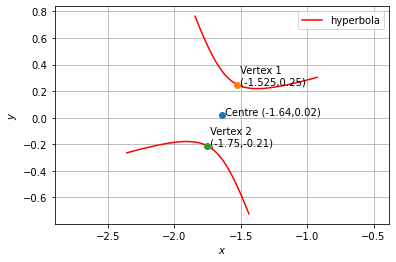
\includegraphics[width=\columnwidth]{./solutions/40/6/hyper.png}
	\caption{} \label{eq:solutions/40/6/linefig1}
\end{figure}

%
\item Find the asymptotes of the hyperbola given below and also the equations to their conjugate hyperbolas.\\
$8x^2+10xy-3y^2-2x+4y-2=0$
%
\solution
The above equation can be expressed in the form 
\begin{align}
\vec{x}^T\vec{V}\vec{x}+2\vec{u}^T\vec{x}+f&=0
%\label{eq:solutions/40/7/2.2} 
\label{eq:solutions/40/7/eq1}
\intertext{Comparing equation we get}
    \vec{V}=\vec{V}^T&=\myvec{8 & 5 \\ 5 &-3}\label{eq:solutions/40/7/eqv}\\
    \vec{u}&=\myvec{-1 \\2 }\label{eq:solutions/40/7/equ}\\
    f&=-2\label{eq:solutions/40/7/eqfv}
\end{align}   
Expanding the Determinant of $\vec{V}$.
\begin{align}
    \Delta_{V} &= \begin{array}{|cc|}
8 &5\\5 & -3
\end{array}<0\label{eq:solutions/40/7/eq:hyp}
\end{align}
Hence from \eqref{eq:solutions/40/7/eq:hyp} given
equation represents the hyperbola
The characteristic equation of $\vec{V}$ is obtained by evaluating the determinant 
\begin{align}
       \begin{array}{|c|}
V-\lambda\vec{I}
\end{array}&=0\\
   \begin{array}{|cc|}
8-\lambda & 5 \\ 5 & -3-\lambda
\end{array}&=0\\
    \brak{8-\lambda}\brak{-3-\lambda}-25=0\\
    \lambda_{1}= \frac{5+\sqrt{221}}{2}\label{eq:solutions/40/7/eq:matrix_l1}\\
    \lambda_{2}= \frac{5-\sqrt{221}}{2}\label{eq:solutions/40/7/eq:matrix_l2}
\end{align}
The eigenvector $\vec{p}$ is defined as 
\begin{align}
    \vec{V}\vec{p}&=\lambda\vec{p}\\
    \implies (\vec{V}-\lambda\vec{I})\vec{p}&=0\label{eq:solutions/40/7/eq:7/eqev}
\end{align}
For $\lambda_1=\frac{5+\sqrt{221}}{2}$ ,
\begin{align}
    (\vec{V}-\lambda_1\vec{I})=\myvec{\frac{11-\sqrt{221}}{2} & 5 \\5 & \frac{-11-\sqrt{221}}{2}}
\end{align}
By row reduction , 
\begin{align}
    &\myvec{\frac{11-\sqrt{221}}{2} & 5 \\5 & \frac{-11-\sqrt{221}}{2}}\\
    %&\xleftrightarrow{\frac{R_1}{\frac{\sqrt{533}+2}{2}}}\\
    &\xleftrightarrow{R_1\leftarrow R_2}
    \myvec{\frac{-11-\sqrt{221}}{2} & 5 \\ \frac{11-\sqrt{221}}{2} & 5}\\
 &\xleftrightarrow{R_2\leftarrow R_2-\frac{11-\sqrt{221}}{10}R_{1}}
    \myvec{5 & \frac{-11-\sqrt{221}}{2} \\ 0& 0}\\
     &\xleftrightarrow{R_1\leftarrow R_1/5}
    \myvec{1 & \frac{-11-\sqrt{221}}{10} \\ 0& 0}
    \label{eq:solutions/40/7/eq:7/eqs1}
\end{align}
Subsituting equation \ref{eq:solutions/40/7/eq:7/eqs1} in equation \ref{eq:solutions/40/7/eq:7/eqev} we get
\begin{align}
        & \myvec{1 & \frac{-11-\sqrt{221}}{10} \\ 0& 0}\myvec{v_1 \\ v_2}=\myvec{0 \\ 0}\label{eq:solutions/40/7/eq:7/eqei1}
\end{align}
Where, $\vec{p}=\myvec{v_1\\v_2}$
Let $v_2=t$
\begin{align}
    v_1&=\frac{t(11+\sqrt{221})}{10}
\end{align}
Eigen vector $\vec{p_1}$ is given by
\begin{align}
    \vec{p_1}&=\myvec{\frac{t(11+\sqrt{221})}{10} \\ t}
\end{align}
Let $t=1$, we get
\begin{align}
        \vec{p_1}&=\myvec{\frac{11+\sqrt{221}}{10} \\1 }\label{eq:solutions/40/7/eq:es71/eqp1}
\end{align}
For $\lambda_2=\frac{5-\sqrt{221}}{2}$ ,
\begin{align}
    (\vec{V}-\lambda_2\vec{I})=\myvec{\frac{11+\sqrt{221}}{2} & 5 \\5 & \frac{-11+\sqrt{221}}{2}}
\end{align}
By row reduction , 
\begin{align}
     \myvec{\frac{11+\sqrt{221}}{2} & 5 \\5 & \frac{-11+\sqrt{221}}{2}}
    \xleftrightarrow{R_1\leftarrow R_2+ \frac{11-\sqrt{221}}{10}R_1}
     \myvec{\frac{11+\sqrt{221}}{2} &5\\ 0& 0}\\  
 \xleftrightarrow{R_1\leftarrow
 \frac{R_1}{\frac{11+\sqrt{221}}{10}}}
    \myvec{1 & \frac{10}{11+\sqrt{221}} \\ 0& 0}
    \label{eq:solutions/40/7/eq:es71/eqs2}
\end{align} 
Substiuting equation \ref{eq:solutions/40/7/eq:es71/eqs2} in equation \ref{eq:solutions/40/7/eq:7/eqev} we get 
\begin{align}
    &\myvec{1 & \frac{10}{11+\sqrt{221}} \\0 & 0}\myvec{v_1 \\ v_2}=\myvec{0 \\ 0}
%\label{eq:solutions/40/7/eq:es71/eqei1}
\end{align}
Where, $\vec{p}=\myvec{v_1\\v_2}$
Let $v_2=t$
\begin{align}
    v_1&=\frac{-t\brak{10}}{11+\sqrt{221}}
\end{align}
Eigen vector $\vec{p_2}$ is given by
\begin{align}
        \vec{p_2}&=\myvec{\frac{-t\brak{10}}{11+\sqrt{221}} \\ t}
\end{align}
Let $t=1$, we get 
\begin{align}
    \vec{p_2}&=\myvec{\frac{\brak{-10}}{11+\sqrt{221}} \\1 }\label{eq:solutions/40/7/eq:es71/eqp2}
\end{align}
By eigen decompostion $\vec{V}$ can be represented by
\begin{align}
    \vec{V}&=\vec{P}\vec{D}\vec{P}^T\label{eq:solutions/40/7/eq:es71/eqsubs}
\end{align}
where 
\begin{align}
        \vec{P}&=\myvec{\vec{p_1} & \vec{p_2}}\label{eq:solutions/40/7/eq:es71/eqp}\\
    \vec{D}&=\myvec{\lambda_1 & 0 \\0 & \lambda_2}\label{eq:solutions/40/7/eq:es71/eqD}
\end{align}
Substituting equations \ref{eq:solutions/40/7/eq:es71/eqp1}, \ref{eq:solutions/40/7/eq:es71/eqp2} in equation \ref{eq:solutions/40/7/eq:es71/eqp} we get 
\begin{align}
    \vec{P}&=\myvec{\frac{11+\sqrt{221}}{10} & \frac{-10}{11+\sqrt{221}} \\1 & 1}\label{eq:solutions/40/7/eq:es71/eqP}
\end{align}
Substituting equations \ref{eq:solutions/40/7/eq:matrix_l1}, \ref{eq:solutions/40/7/eq:matrix_l2} in \ref{eq:solutions/40/7/eq:es71/eqD} we get
\begin{align}
       \vec{D}&=\myvec{\frac{5+\sqrt{221}}{2} & 0\\0 & \frac{5-\sqrt{221}}{2}}\label{eq:solutions/40/7/eq:es71/eqDD}
\end{align}
Centre of the hyperbola is given by 
\begin{align}
    \vec{c}&=-\vec{V}^{-1}\vec{u}\\
    \implies\vec{c}&=-\myvec{\frac{3}{49}&\frac{5}{49}\\\frac{5}{49}&\frac{-8}{49}}\myvec{-1 \\ 2}\\
    \implies\vec{c}&=\myvec{\frac{-3}{49}&\frac{-5}{49}\\\frac{-5}{49}&\frac{8}{49}}\myvec{-1 \\ 2}\\
    \implies\vec{c}&=\myvec{\frac{-1}{7}\\\frac{3}{7}}
\end{align}
Since,
\begin{align}
    \vec{u}^T\vec{V}^{-1}\vec{u}-f = 1 > 0\label{eq:solutions/40/7/eq:es71/cond}
\end{align} 
there isn't a need to swap axes
In hyperbola,
\begin{align}
axes=
\begin{cases}
\sqrt{\frac{\vec{u}^T\vec{V}^{-1}\vec{u}-f}{\lambda_1}}\\ \sqrt{\frac{f-\vec{u}^T\vec{V}^{-1}\vec{u}}{\lambda_2}}
\end{cases}
\end{align}
From above equations we can say that,
\begin{align}
\sqrt{\frac{\vec{u}^T\vec{V}^{-1}\vec{u}-f}{\lambda_1}}=\sqrt{ \frac{2}{5+\sqrt{221}}}\\
\sqrt{\frac{f-\vec{u}^T\vec{V}^{-1}\vec{u}}{\lambda_2}}=\sqrt{ \frac{2}{5-\sqrt{221}}}
\end{align}
Now we have,
\begin{align}
    \vec{y}^T\vec{D}\vec{y}&=\vec{u}^T\vec{V}^{-1}\vec{u}-f\label{eq:solutions/40/7/eq:es71/fi}
\end{align}
where ,
\begin{align}
    \vec{y}&=\vec{P}^T(\vec{x}-\vec{c})
\end{align}
To get $\vec{y}$,
\begin{align}
\vec{y}&=\vec{P}^T\vec{x}-\vec{P}^T\vec{c}\\
    \vec{y}&= \myvec{\frac{11+\sqrt{221}}{10} & 1 \\ \frac{-10}{11+\sqrt{221}} & 1}\vec{x}-\myvec{\frac{11+\sqrt{221}}{10} & 1 \\ \frac{-10}{11+\sqrt{221}} & 1}\myvec{\frac{-1}{7}\\\frac{3}{7}}\\
    \vec{y}&=\myvec{\frac{11+\sqrt{221}}{10} & 1 \\ \frac{-10}{11+\sqrt{221}} & 1}\vec{x}-\myvec{\frac{-11-\sqrt{221}}{70}+\frac{3}{7} \\ \frac{10}{(7)11+(7)\sqrt{221}}+\frac{3}{7}}
\end{align}
Subsituting the eqauations \eqref{eq:solutions/40/7/eq:es71/cond}, \eqref{eq:solutions/40/7/eq:es71/eqDD} in equation \eqref{eq:solutions/40/7/eq:es71/fi}
\begin{align}
   \implies\vec{y}^T\myvec{\frac{5+\sqrt{221}}{2} & 0 \\0 & \frac{5-\sqrt{221}}{2}}\vec{y}+2&=0
\end{align}
{Asymptotes of hyperbola}
Equation of a hyperbola and the combined equation of the Asymptotes differ only in the constant term.
\begin{align}
 8x^2+10xy-3y^2-2x+4y+K=0   
\end{align}
The above equation can be expressed in the form 
\begin{align}
\vec{x}^T\vec{V}\vec{x}+2\vec{u}^T\vec{x}+f&=0
%\label{eq:solutions/40/7/2.2} 
%\label{eq:solutions/40/7/eq1}
\intertext{Comparing equation we get}
    \vec{V}=\vec{V}^T&=\myvec{8 & 5 \\ 5 &-3}\label{eq:solutions/40/7/es1/eqv}\\
    \vec{u}&=\myvec{-1 \\2 }\label{eq:solutions/40/7/eq:equ}\\
    f&=K\label{eq:solutions/40/7/eq:es1/eqfv}
\end{align}   
\begin{align}
\Delta&=\begin{array}{|ccc|}
8 & 5 & -1\\ 5& -3 & 2\\ -1 & 2 & K
\end{array}\\
\implies K&=-1
\end{align}
Similar way expanding the Determinant of $\vec{V}$.
\begin{align}
    \Delta_{V} &= \begin{array}{|cc|}
8 &5\\5 & -3
\end{array}<0\label{eq:solutions/40/7/eq:es/17/hyp}
\end{align}
From \eqref{eq:solutions/40/7/eq:es/17/hyp} we could say that the given equation represents two straight lines
Let the equations of lines be,
\begin{align}
	\brak{\vec{n_1}^T \vec{x} - c_1}\brak{\vec{n_1}^T \vec{x} - c_1} =
        \vec{x}^{T}\vec{Vx} + 2\vec{u}^{T}\vec{x} + f=0\label{eq:solutions/40/7/eq:eql7/03}
\end{align}
\begin{align}
\brak{\vec{n_1}^T\vec{x}-c_1}\brak{\vec{n_2}^T\vec{x}-c_2}
&=\vec{x}^T\myvec{8 & 5 \\ 5 & -3}\vec{x}\notag\\
+2\myvec{-1 & 2}\vec{x}-1\label{eq:solutions/40/7/equate}\\
    \vec{n_1}*\vec{n_2} = \myvec{a\\2b\\c} &= \myvec{8\\10\\-3}\label{eq:solutions/40/7/conv}\\
    c_2\vec{n_1}+c_1\vec{n_2}&=-2\myvec{-1\\2}\label{eq:solutions/40/7/eq17/c1c2}\\
    c_1c_2&=-1
\end{align}
The slopes of the lines are given by the roots of the polynomial 
\begin{align}
    &cm^2+2bm+a=0\label{eq:solutions/40/7/e}\\
    \implies m_i&=\frac{-b\pm{\sqrt{-\Delta_{V}}}}{c}\\
    \vec{n_i}&=k\myvec{-m_i\\1}
\end{align}
Substituting the given data in above equations \eqref{eq:solutions/40/7/e} we get,
\begin{align}
    &-3m^2+10m+8=0\\
    m_1&=4,  m_2=\frac{-2}{3}\\
   &= \vec{n_1}=\myvec{-4\\ 1}, \vec{n_2}=\myvec{-2\\-3} \label{eq:solutions/40/7/eq:normal1}
\intertext{We know that,}
& \vec{n_1}\ast \vec{n_2} = \myvec{a\\2b\\c} \label{eq:solutions/40/7/eq:conv1}
\end{align}
Verification using Toeplitz matrix, From equation \eqref{eq:solutions/40/7/eq:normal1}
\begin{align}
    \vec{n_1}=\myvec{-4&0\\1&-4\\0&-1}
    \vec{n_2}=\myvec{-2\\-3}\label{eq:solutions/40/7/eq:conv2}\\
\implies \myvec{-4&0\\1&-4\\0&1}\myvec{0\\ -1} = \myvec{8\\10\\-3} = \myvec{a\\2b\\c}\label{eq:solutions/40/7/eq:conv3}
\end{align}
$\implies$ Equation \eqref{eq:solutions/40/7/eq:normal1} satisfies \eqref{eq:solutions/40/7/eq:conv1}\\
$c_1$ and $c_2$ can be obtained as,
\begin{align}
\myvec{\vec{n_1} & \vec{n_2}}\myvec{c_2\\c_1}&=-2\vec{u} \label{eq:solutions/40/7/eq:aug1}
\end{align}
Substituting \eqref{eq:solutions/40/7/eq:normal1} in \eqref{eq:solutions/40/7/eq:aug1}, the augmented matrix is,
\begin{align}
\myvec{-4 & -2 & -2 \\ 1 & -3 & 4}
\xleftrightarrow[R_2\leftarrow R_2-R_1]{R_1\leftarrow -R_1/4}
\myvec{1 &\frac{1}{2} &\frac{1}{2} \\ 0 & -\frac{7}{2} & \frac{7}{2}} \label{eq:solutions/40/7/eq:aug5}\\
\xleftrightarrow[R_1\leftarrow R_1-\frac{1}{2}R_2]{R_2\leftarrow -\frac{2}{7}R_2}
\myvec{1 &0 &1 \\ 0& 1 & -1} \label{eq:solutions/40/7/eq:aug2}\\
\implies c_1 = 1, c_2=-1 \label{eq:solutions/40/7/eq:const1}
\end{align}
Equations \eqref{eq:solutions/40/7/eq:eql7/03}, can be modified as,from \eqref{eq:solutions/40/7/eq:normal1} and \eqref{eq:solutions/40/7/eq:const1} in we get,
\begin{align}
    \myvec{-4 & 1}\vec{x}&=1\\
    \myvec{-2 & -3}\vec{x}&=-1
\end{align}
\begin{multline}
\implies \brak{-4x+y-1}\brak{-2x-3y+1}= 0\\
\implies \boxed{\brak{4x-y+1}\brak{2x+3y-1} = 0} \label{eq:solutions/40/7/eq:line1}
\end{multline}
The angle between the lines can be expressed as, 
\begin{align}
	\vec{n_1}=\myvec{-4\\1} , \quad \vec{n_2}=\myvec{-2\\-3}\\
	\cos\theta=\frac{\vec{n_1}^T\vec{n_2}}{\norm{\vec{n_1}}\norm{\vec{n_2}}} \\
	\implies \quad \theta=\cos^{-1}({\frac{0}{\sqrt{221}}}) = 90\degree.
\end{align}
{Equation of Asymptotes: }
The characteristic equation of $\vec{V}$ is obtained by evaluating the determinant \eqref{eq:solutions/40/7/es1/eqv}
\begin{align}
       \begin{array}{|c|}
V-\lambda\vec{I}
\end{array}&=0\\
   \begin{array}{|cc|}
8-\lambda & 5 \\ 5 & -3-\lambda
\end{array}&=0\\
    \brak{8-\lambda}\brak{-3-\lambda}-25=0\\
    \lambda_{1}= \frac{5+\sqrt{221}}{2}\\
    \lambda_{2}= \frac{5-\sqrt{221}}{2}
\end{align}
The eigenvector $\vec{p}$ is defined as 
\begin{align}
    \vec{V}\vec{p}&=\lambda\vec{p}\\
    \implies (\vec{V}-\lambda\vec{I})\vec{p}&=0\label{eq:solutions/40/7/eq:es/2701}
\end{align}
For $\lambda_1=\frac{5+\sqrt{221}}{2}$ ,
\begin{align}
    (\vec{V}-\lambda_1\vec{I})=\myvec{\frac{11-\sqrt{221}}{2} & 5 \\5 & \frac{-11-\sqrt{221}}{2}}
\end{align}
By row reduction , 
\begin{align}
    &\myvec{\frac{11-\sqrt{221}}{2} & 5 \\5 & \frac{-11-\sqrt{221}}{2}}\\
    %&\xleftrightarrow{\frac{R_1}{\frac{\sqrt{533}+2}{2}}}\\
    &\xleftrightarrow{R_1\leftarrow R_2}
    \myvec{\frac{-11-\sqrt{221}}{2} & 5 \\ \frac{11-\sqrt{221}}{2} & 5}\\
 &\xleftrightarrow{R_2\leftarrow R_2-\frac{11-\sqrt{221}}{10}R_{1}}
    \myvec{5 & \frac{-11-\sqrt{221}}{2} \\ 0& 0}\\
     &\xleftrightarrow{R_1\leftarrow R_1/5}
    \myvec{1 & \frac{-11-\sqrt{221}}{10} \\ 0& 0}
    \label{eq:solutions/40/7/eq:es27/02}
\end{align}
Subsituting equation \ref{eq:solutions/40/7/eq:es27/02} in equation \ref{eq:solutions/40/7/eq:es/2701} we get
\begin{align}
        & \myvec{1 & \frac{-11-\sqrt{221}}{10} \\ 0& 0}\myvec{v_1 \\ v_2}=\myvec{0 \\ 0}\label{eq:solutions/40/7/eq:es27/eqei1}
\end{align}
Where, $\vec{p}=\myvec{v_1\\v_2}$
Let $v_2=t$
\begin{align}
    v_1&=\frac{t(11+\sqrt{221})}{10}
\end{align}
Eigen vector $\vec{p_1}$ is given by
\begin{align}
    \vec{p_1}&=\myvec{\frac{t(11+\sqrt{221})}{10} \\ t}
\end{align}
Let $t=1$, we get
\begin{align}
        \vec{p_1}&=\myvec{\frac{11+\sqrt{221}}{10} \\1 }\label{eq:solutions/40/7/eq:es27/eqp1}
\end{align}
For $\lambda_2=\frac{5-\sqrt{221}}{2}$ ,
\begin{align}
    (\vec{V}-\lambda_2\vec{I})=\myvec{\frac{11+\sqrt{221}}{2} & 5 \\5 & \frac{-11+\sqrt{221}}{2}}
\end{align}
By row reduction , 
\begin{align}
    \myvec{\frac{11+\sqrt{221}}{2} & 5 \\5 & \frac{-11+\sqrt{221}}{2}}
    \xleftrightarrow{R_1\leftarrow R_2+ \frac{11-\sqrt{221}}{10}R_1}
     \myvec{\frac{11+\sqrt{221}}{2} &5\\ 0& 0}\\  
 \xleftrightarrow{R_1\leftarrow
 \frac{R_1}{\frac{11+\sqrt{221}}{10}}}
    \myvec{1 & \frac{10}{11+\sqrt{221}} \\ 0& 0}
    \label{eq:solutions/40/7/eq:es27eqs02}
\end{align}
Subsituting equation \ref{eq:solutions/40/7/eq:es27eqs02} in equation \ref{eq:solutions/40/7/eq:es/2701} we get 
\begin{align}
    &\myvec{1 & \frac{10}{11+\sqrt{221}} \\0 & 0}\myvec{v_1 \\ v_2}=\myvec{0 \\ 0}
%\label{eq:solutions/40/7/eq:es27/eqei1}
\end{align}
Where, $\vec{p}=\myvec{v_1\\v_2}$
Let $v_2=t$
\begin{align}
    v_1&=\frac{-t\brak{10}}{11+\sqrt{221}}
\end{align}
Eigen vector $\vec{p_2}$ is given by
\begin{align}
        \vec{p_2}&=\myvec{\frac{-t\brak{10}}{11+\sqrt{221}} \\ t}
\end{align}
Let $t=1$, we get 
\begin{align}
    \vec{p_2}&=\myvec{\frac{\brak{-10}}{11+\sqrt{221}} \\1 }\label{eq:solutions/40/7/eq:es27/eqp2}
\end{align}
By eigen decompostion $\vec{V}$ can be represented by
\begin{align}
    \vec{V}&=\vec{P}\vec{D}\vec{P}^T\label{eq:solutions/40/7/eq:es27/eqsubs}
\end{align}
where 
\begin{align}
        \vec{P}&=\myvec{\vec{p_1} & \vec{p_2}}\label{eq:solutions/40/7/eq:es27/eqp}\\
    \vec{D}&=\myvec{\lambda_1 & 0 \\0 & \lambda_2}\label{eq:solutions/40/7/eq:es27/eqD}
\end{align}
Substituting equations \ref{eq:solutions/40/7/eq:es27/eqp1}, \ref{eq:solutions/40/7/eq:es27/eqp2} in equation \ref{eq:solutions/40/7/eq:es27/eqp} we get 
\begin{align}
    \vec{P}&=\myvec{\frac{11+\sqrt{221}}{10} & \frac{-10}{11+\sqrt{221}} \\1 & 1}\label{eq:solutions/40/7/eq:es27/eqP}
\end{align}
\begin{align}
       \vec{D}&=\myvec{\frac{5+\sqrt{221}}{2} & 0\\0 & \frac{5-\sqrt{221}}{2}}\label{eq:solutions/40/7/eq:es27/eqDD}
\end{align}
Centre of the hyperbola is given by 
\begin{align}
    \vec{c}&=-\vec{V}^{-1}\vec{u}\\
    \implies\vec{c}&=-\myvec{\frac{3}{49}&\frac{5}{49}\\\frac{5}{49}&\frac{-8}{49}}\myvec{-1 \\ 2}\\
    \implies\vec{c}&=\myvec{\frac{-3}{49}&\frac{-5}{49}\\\frac{-5}{49}&\frac{8}{49}}\myvec{-1 \\ 2}\\
    \implies\vec{c}&=\myvec{\frac{-1}{7}\\\frac{3}{7}}
\end{align}
Since,
\begin{align}
    \vec{u}^T\vec{V}^{-1}\vec{u}-f = 0\label{eq:solutions/40/7/eq:es27/cond}
\end{align} 
Now,
\begin{align}
    \vec{y}^T\vec{D}\vec{y}&=\vec{u}^T\vec{V}^{-1}\vec{u}-f\label{eq:solutions/40/7/eq:es27/fi}
\end{align}
where ,
\begin{align}
    \vec{y}&=\vec{P}^T(\vec{x}-\vec{c})
\end{align}
To get $\vec{y}$,
\begin{align}
\vec{y}&=\vec{P}^T\vec{x}-\vec{P}^T\vec{c}\\
    \vec{y}&= \myvec{\frac{11+\sqrt{221}}{10} & 1 \\ \frac{-10}{11+\sqrt{221}} & 1}\vec{x}-\myvec{\frac{11+\sqrt{221}}{10} & 1 \\ \frac{-10}{11+\sqrt{221}} & 1}\myvec{\frac{-1}{7}\\\frac{3}{7}}\\
    \vec{y}&=\myvec{\frac{11+\sqrt{221}}{10} & 1 \\ \frac{-10}{11+\sqrt{221}} & 1}\vec{x}-\myvec{\frac{-11-\sqrt{221}}{70}+\frac{3}{7} \\ \frac{10}{(7)11+(7)\sqrt{221}}+\frac{3}{7}}
\end{align}
Subsituting the eqauations \eqref{eq:solutions/40/7/eq:es27/cond}, \eqref{eq:solutions/40/7/eq:es27/eqDD} in equation \eqref{eq:solutions/40/7/eq:es27/fi}
Equation of asymptotes is
\begin{align}
    \implies \vec{y}^T\myvec{\frac{5+\sqrt{221}}{2} & 0 \\0 & \frac{5-\sqrt{221}}{2}}\vec{y}+1&=0
\end{align}
And the Equations of Conjugate hyperbola is 2(Equation of Asymptotes)- Equation of hyperbola. 
\begin{align}
    \implies \vec{y}^T\myvec{\frac{5+\sqrt{221}}{2} & 0 \\0 & \frac{5-\sqrt{221}}{2}}\vec{y}&=0
\end{align}
\begin{figure}[h]
    \centering
    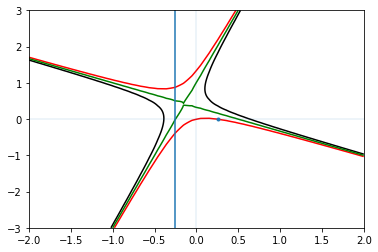
\includegraphics[width=\columnwidth]{./solutions/40/7/figs/A7_4.png}
    \caption{Hyperbola with assymptotes and its conjugate}
    \label{eq:solutions/40/7/Fig :1}
\end{figure}

%
\item What conics do the following equation represents? When possible, find the center and the equation reffered to the center.
\begin{multline}
55x^2 - 120xy + 20y^2 +64x -48y=0
\label{eq:solutions/40/9/eqn1}
\end{multline}
%
\solution
The general equation of second degree can be represented as:
\begin{align}
\vec{X}^T\vec{V}\vec{X} + 2\vec{u}^T\vec{X} + f = 0
\end{align}
The above \ref{eq:solutions/40/9/eqn1} can also be written as:
\begin{align}
\vec{X}^T\myvec{55 & -60\\-60 & 20}\vec{X} + 2\myvec{32 & -24}\vec{X} +0 = 0
\end{align}
So, 
\begin{align}
\vec{V} = \myvec{55 & -60\\-60 & 20}
\end{align}
and 
\begin{align}
\vec{u} = \myvec{32 \\ -24}\\
f=0
\end{align}
Now, 
\begin{align}
\det{\vec{V}} = \mydet{55 & -60\\-60 & 20}\\
\implies \det{\vec{V}} = -2500 <0
\end{align}

As $\det{\vec{V}}<0$, so we can say that the above conic section \ref{eq:solutions/40/9/eqn1} is hyperbola.Now,
\begin{align}
\vec{V}^{-1} =\frac{1}{-2500} \myvec{20 & 60\\60 & 55}
\end{align}
The center of this hyperbola will be:
\begin{align}
\vec{c} = - \vec{V}^{-1} \vec{u}\\
\implies \vec{c} = \frac{1}{2500} \myvec{20 & 60\\60 & 55} \myvec{32 \\ -24}\\
\implies \vec{c} = \myvec{-\frac{8}{25} \\ \frac{6}{25}}\\
\end{align}
 Now the characteristic equation of $\vec{V}$ is obtained as:
\begin{align}
\mydet{\vec{V} - \lambda\vec{I}} =0\\
\implies \mydet{55-\lambda & -60\\-60 & 20-\lambda} = 0\\
\implies \lambda^2 - 75\lambda - 2500=0
\end{align}
The eigen values are given by:
\begin{align}
\lambda_1=100\\
\lambda_2 = -25
\end{align}
The eigen vector $\vec{P}$ is defined as:
\begin{align}
\vec{V}\vec{P} = \lambda \vec{P}\\
\implies (\vec{V} -\lambda\vec{I})\vec{P} = \vec{0}
\end{align}
For $\lambda_1$=100,
\begin{align}
(\vec{V} -\lambda_1\vec{I}) = \myvec{-45 & -60\\-60 & -80}
\end{align}
By row reduction,
\begin{align}
\myvec{-45 & -60\\-60 & -80}\xleftrightarrow[R_1\leftarrow R_1 /(-5)]{R_2\leftarrow R_2/(-5)}\\
\myvec{9 & 12\\12 & 16}\xleftrightarrow[R_1\leftarrow R_1 /3]{R_2\leftarrow R_2/4}\\
\myvec{3 & 4\\3 & 4}\xleftrightarrow[]{R_2\leftarrow R_2-R_1}\myvec{3 & 4\\0 & 0}
\end{align}
So, 
\begin{align}
(\vec{V} -\lambda_1\vec{I})\vec{P_1} = \vec{0}\\
\implies \myvec{3 & 4\\0 & 0} \myvec{v_1\\v_2} = \myvec{0\\0}\\
\implies \vec{P_1} = \myvec{-\frac{4}{3}\\1}
\end{align}
Similarly,
For $\lambda_2$=100,
\begin{align}
(\vec{V} -\lambda_2\vec{I}) = \myvec{80 & -60\\-60 & 45}
\end{align}
By row reduction,
\begin{align}
\myvec{80 & -60\\-60 & 45}\xleftrightarrow[R_1\leftarrow R_1 /5]{R_2\leftarrow R_2/5}\\
\myvec{16 & -12\\-12 & 9}\xleftrightarrow[R_1\leftarrow R_1 /4]{R_2\leftarrow R_2/(-3)}\\
\myvec{4 & -3\\4 & -3}\xleftrightarrow[]{R_2\leftarrow R_2-R_1}\myvec{4 & -3\\0 & 0}
\end{align}
So, 
\begin{align}
(\vec{V} -\lambda_2\vec{I})\vec{P_2} = \vec{0}\\
\implies \myvec{4 & -3\\0 & 0} \myvec{v_1\\v_2} = \myvec{0\\0}\\
\implies \vec{P_2} = \myvec{1\\ \frac{4}{3}}
\end{align}
By eigen decomposition $\vec{V}$ can also be written as:
\begin{align}
\vec{V} = \vec{P}\vec{D}\vec{P}^T
\end{align}
where 
\begin{align}
\vec{P} = \myvec{\vec{P_1} & \vec{P_2}}\\
\vec{D} =\myvec{\lambda_1 & 0\\0 & \lambda_2}
\end{align}
So, 
\begin{align}
\vec{P} = \myvec{-\frac{4}{3} & 1\\1 & \frac{4}{3}}\\
\vec{D} =\myvec{100 & 0\\0 & -25}
\end{align}
and 
\begin{align}
\vec{u}^T\vec{V}^{-1}\vec{u}-f=16>0
\end{align}
So, the axes are:
\begin{align}
a=\sqrt{\frac{\vec{u}^T\vec{V}^{-1}\vec{u}-f}{\lambda_1}} = \frac{2}{5}\\
b=\sqrt{\frac{f-\vec{u}^T\vec{V}^{-1}\vec{u}}{\lambda_2}} = \frac{4}{5}
\end{align}
Now, the equation \ref{eq:solutions/40/9/eqn1} can be written as:
\begin{align}
\vec{y}^T\vec{D}\vec{y}=\vec{u}^T\vec{V}^{-1}\vec{u}-f
\end{align}
where, 
\begin{align}
\vec{y}= \vec{P}^T (\vec{x}-\vec{c})
\end{align}
So, 
\begin{align}
\vec{y}^T\myvec{100 & 0\\0 & -25}\vec{y}=16\\
\implies \vec{y}^T\myvec{100 & 0\\0 & -25}\vec{y}-16=0
\end{align}

\begin{figure}[!ht]
\centering
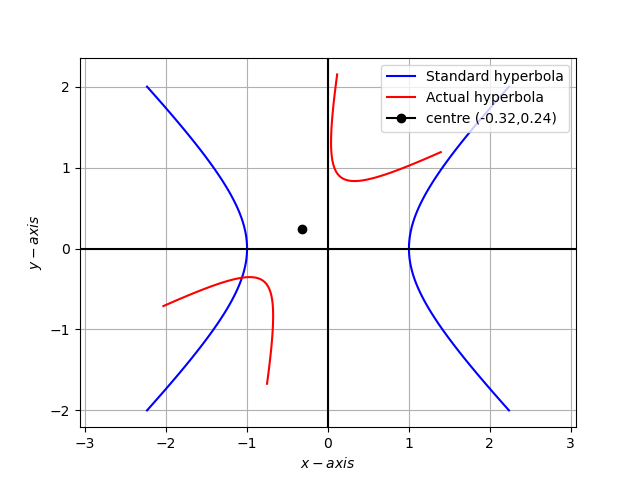
\includegraphics[width=\columnwidth]{./solutions/40/9/figs/hyperbola_2.png}
\caption{Comparison of the Standerd and Actual Hyperbola}
\label{eq:solutions/40/9/fig:hyperbola}
\end{figure}





%
\item  Find the asymptotes of the given hyperbola and also the equation to its conjugate hyperbola
\begin{align}
19x^2 + 24xy+y^2-22x-6y=0 \label{eq:solutions/40/10/1.1}
\end{align}
%
\solution
The general equation of second degree is given by
\begin{align}
ax^2+2bxy+cy^2+2dx+2ey+f=0\label{eq:solutions/40/10/2.1}
\end{align}
and can be expressed as
\begin{align}
\vec{x}^T\vec{V}\vec{x}+2\vec{u}^T\vec{x}+f=0 \label{eq:solutions/40/10/2.2}
\end{align}
where
\begin{align}
\vec{V} &= \vec{V}^T = \myvec{a & b \\ b & c}
\\
\vec{u} &= \myvec{d \\ e}
\intertext{Comparing equations \ref{eq:solutions/40/10/1.1} and \ref{eq:solutions/40/10/2.2} we get}
    \vec{V}=\vec{V}^T&=\myvec{19 & 12 \\ 12 &1}\label{eq:solutions/40/10/2.5}\\
    \vec{u}&=\myvec{-11 \\-3 }\label{eq:solutions/40/10/2.6}\\
    f&=0\label{eq:solutions/40/10/2.7}
\end{align}   
Expanding the Determinant of $\vec{V}$.
\begin{align}
    \Delta_{V} &= \begin{array}{|cc|}
19 &12\\12 & 1
\end{array}<0\label{eq:solutions/40/10/2.8}
\end{align}
Hence from \ref{eq:solutions/40/10/2.8} given
equation represents the hyperbola.\\
The characteristic equation of $\vec{V}$ is obtained by evaluating the determinant 
\begin{align}
       \begin{array}{|c|}
V-\lambda\vec{I}
\end{array}&=0\\
   \begin{array}{|cc|}
19-\lambda & 12 \\ 12 & 1-\lambda
\end{array}&=0\\
    \brak{19-\lambda}\brak{1-\lambda}-144=0\\
    \lambda_{1}=-5,   \lambda_{2}= 25 \label{eq:solutions/40/10/2.12}
\end{align}
The eigenvector $\vec{p}$ is defined as 
\begin{align}
    \vec{V}\vec{p}&=\lambda\vec{p}\\
    \implies (\vec{V}-\lambda\vec{I})\vec{p}&=0\label{eq:solutions/40/10/2.14}
\end{align}
For $\lambda_1=-5$ ,
\begin{align}
    (\vec{V}-\lambda_1\vec{I})=\myvec{19+5 & 12 \\12 & 1+5}
\end{align}
By row reduction , 
\begin{align}
    &\myvec{24 & 12 \\12 & 6}\\
&\xleftrightarrow{R_2\leftarrow 2R_2 -R_1}
    \myvec{24 & 12 \\ 0& 0}\\
        &\xleftrightarrow{R_1\leftarrow \frac{R_1}{12}}
    \myvec{2 & 1 \\ 0& 0}
    \label{eq:solutions/40/10/2.18}
\end{align}
Subsituting equation \ref{eq:solutions/40/10/2.18} in equation \ref{eq:solutions/40/10/2.14} we get
\begin{align}
        &   \myvec{2 & 1 \\ 0& 0}\myvec{u_1 \\ u_2}=\myvec{0 \\ 0}\label{eq:solutions/40/10/2.19}
\end{align}
Where, $\vec{p}=\myvec{u_1\\u_2}$
Let $u_1=t$
\begin{align}
    u_2&=-2t
\end{align}
Eigen vector $\vec{p_1}$ is given by
\begin{align}
    \vec{p_1}&=\myvec{t \\ -2t}
\end{align}
Let $t=1$, we get
\begin{align}
        \vec{p_1}&=\myvec{1 \\-2 }\label{eq:solutions/40/10/2.22}
\end{align}
For $\lambda_2=25$ ,
\begin{align}
    (\vec{V}-\lambda_2\vec{I})=\myvec{19-25 & 12 \\12 & 1-25}
\end{align}
By row reduction , 
\begin{align}
    &\myvec{-6 & 12 \\12 & -24}\\
&\xleftrightarrow{R_2\leftarrow R_2 +2R_1}
    \myvec{-6 & 12 \\ 0& 0}\\
        &\xleftrightarrow{R_1\leftarrow \frac{R_1}{6}}
    \myvec{-1 & 2 \\ 0& 0}
    \label{eq:solutions/40/10/2.26}
\end{align}
Subsituting equation \ref{eq:solutions/40/10/2.26} in equation \ref{eq:solutions/40/10/2.14} we get
\begin{align}
        &   \myvec{-1 & 2 \\ 0& 0}\myvec{v_1 \\ v_2}=\myvec{0 \\ 0}\label{eq:solutions/40/10/2.27}
\end{align}
Where, $\vec{p}=\myvec{v_1\\v_2}$
Let $v_1=t$
\begin{align}
    v_2&=\frac{t}{2}
\end{align}
Eigen vector $\vec{p_2}$ is given by
\begin{align}
    \vec{p_2}&=\myvec{t \\ \frac{t}{2}}
\end{align}
Let $t=1$, we get
\begin{align}
        \vec{p_2}&=\myvec{1 \\\frac{1 }{2}}\label{eq:solutions/40/10/2.30}
\end{align}
By eigen decompostion $\vec{V}$ can be represented by
\begin{align}
    \vec{V}&=\vec{P}\vec{D}\vec{P}^T\label{eq:solutions/40/10/2.31}
\end{align}
where 
\begin{align}
        \vec{P}&=\myvec{\vec{p_1} & \vec{p_2}}\label{eq:solutions/40/10/2.32}\\
    \vec{D}&=\myvec{\lambda_1 & 0 \\0 & \lambda_2}\label{eq:solutions/40/10/2.33}
\end{align}

Substituting equations \ref{eq:solutions/40/10/2.22}, \ref{eq:solutions/40/10/2.30} in equation \ref{eq:solutions/40/10/2.32} we get 
\begin{align}
    \vec{P}&=\myvec{1 & 1 \\-2 & \frac{1}{2}}\label{eq:solutions/40/10/2.34}
\end{align}
Substituting equation \ref{eq:solutions/40/10/2.12} in \ref{eq:solutions/40/10/2.33} we get
\begin{align}
       \vec{D}&=\myvec{-5 & 0\\0 & 25}\label{eq:solutions/40/10/2.35}
\end{align}
Equation of a hyperbola and the combined equation of the Asymptotes differ only in the constant term.
\begin{align}
 19x^2 + 24xy+y^2-22x-6y+K=0   \label{eq:solutions/40/10/2.36}
\end{align}
The above equation can be expressed in the form 
\begin{align}
\vec{x}^T\vec{V}\vec{x}+2\vec{u}^T\vec{x}+f&=0 \label{eq:solutions/40/10/2.37}
\intertext{Comparing equation we get}
    \vec{V}=\vec{V}^T&=\myvec{19 & 12 \\ 12 &1}\label{eq:solutions/40/10/2.38}\\
    \vec{u}&=\myvec{-11 \\-3 }\label{eq:solutions/40/10/2.39}\\
    f&=K\label{eq:solutions/40/10/2.40}
\end{align}
\begin{align}
\Delta&=\begin{array}{|ccc|}19 & 12 & -11\\ 12& 1 & -3\\ -11 & -3 & K
\end{array}
\end{align}
Since the equations represent pair of straight lines, equating the determinant to zero, we can get the value of K
\begin{align}
\implies K=4 \label{eq:solutions/40/10/2.42}
\end{align}
Let $(\alpha,\beta)$ be their point of intersection, then
\begin{equation}\label{eq:solutions/40/10/2.43}
	\myvec{ a & b\\ b & c}\myvec{\alpha \\ \beta} = \myvec{-d \\ -e}
\end{equation}
Substituting the values, we obtain,
\begin{align}
\myvec{19 & 12 \\ 12 &1}\myvec{\alpha \\ \beta} = \myvec{11 \\ 3}\\
\text{We get, } \alpha =  \frac{1}{5} , \beta = \frac{3}{5}
\end{align}

Using Affine transformation and Spectral decomposition, we get
\begin{align}
X^\prime = \pm \sqrt{-\frac{\lambda_2}{\lambda_1}}Y^\prime\\
\text{where } X^\prime = Xu_1 + Yu_2 \\
Y^\prime = Xv_1 + Yv_2\\
X = x-\alpha \text{ and } Y = y - \beta
\end{align}
Therefore, 
\begin{multline}
	u_1(x-\alpha) + u_2(y-\beta) = \\ \pm \sqrt{-\frac{\lambda_2}{\lambda_1}}(v_1(x-\alpha) + v_2(y-\beta))  
%\label{eq:solutions/40/10/2.57}
\end{multline}
Substituting values, we get 
\begin{multline}
	(x-\frac{1}{5})-2(y-\frac{3}{5}) = \\ \pm \sqrt{\frac{25}{5}}(x-\frac{1}{5})+\frac{1}{2}(y-\frac{3}{5}) 
\end{multline}
Simplifying above equation
\begin{align}
	8x+ 9y - 7 = 0 \\
	12x + y + 7 = 0\\
	\implies (8x+ 9y - 7 )(12x + y + 7) = 0
\end{align}
Thus the equation of lines are
\begin{align}
	\myvec{8 & 9}\vec{x} = 7 \\
	\myvec{12 & 1}\vec{x} = -7 
\end{align}

 The Equation of Conjugate hyperbola is given by:\\
\\
2(Equation of Asymptotes)- Equation of hyperbola.\\
\\
From Eq \ref{eq:solutions/40/10/1.1} and \ref{eq:solutions/40/10/2.36}, we obtain equation of Conjugate hyperbola as:-
\begin{align}
19x^2 + 24xy+y^2-22x-6y+8=0  \label{eq:solutions/40/10/2.57}
\end{align}
The general equation of second degree is given by
\begin{align}
ax^2+2bxy+cy^2+2dx+2ey+f=0\label{eq:solutions/40/10/2.59}
\end{align}
comparing equation \ref{eq:solutions/40/10/2.57} with the general equation of second degree given at \ref{eq:solutions/40/10/2.59}, it can be expressed as
\begin{align}
\vec{x}^T\vec{V}\vec{x}+2\vec{u}^T\vec{x}+f=0 \label{eq:solutions/40/10/2.58}
\end{align}
where
\begin{align}
\vec{V} &= \vec{V}^T = \myvec{a & b \\ b & c}
\\
\vec{u} &= \myvec{d\\ e}
\intertext{Comparing equations \ref{eq:solutions/40/10/2.57} and \ref{eq:solutions/40/10/2.58} we get}
    \vec{V}=\vec{V}^T&=\myvec{19 & 12 \\ 12 &1}\\
    \vec{u}&=\myvec{-11 \\-3 }\\
    f&=8
\end{align}   
Therefore, the equation of the conjugate hyperbola is as given below:-
\begin{align}
\vec{x}^T\myvec{19 & 12 \\12 & 1}\vec{x} +2\myvec{-11 & -3} \vec{x}&+8= 0 \label{eq:solutions/40/10/2.66}
\end{align}

\begin{figure}[h]
    \centering
    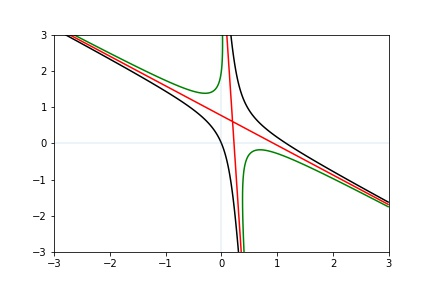
\includegraphics[width=\columnwidth]{./solutions/40/10/hyperbola.jpg}
    \caption{Hyperbola, Conjugate Hyperbola and Asymptotes}
    \label{eq:solutions/40/10/Fig :1}
\end{figure}

\end{enumerate}


